\section{同调恢复}
\label{sec:mrec-homology-recovery}

前几节恢复的都是局部的量。流形有几个分支、有几个洞，是整体的拓扑信息，单看任何一个邻域都无法知道。第~\ref{chap:homology}章用同调空间的维数，即Betti数，记录这类信息：$\beta_0$是连通分支数，圆的$\beta_1=1$对应绕一圈的环。本节研究怎样只用有限样本算出底层流形的同调。

路线分三步。先把离散的样本加粗成连续的空间，即以样本为球心的球并；再用有限的组合数据记录球与球怎样交叠，得到Čech复形与Rips复形；最后用神经引理和形变收缩证明，在适当的尺度下，复形的同调等于流形的同调。整个论证得到的是同伦等价与同调同构，不是同胚，更不是光滑结构的恢复。

\subsection{样本的球并}
\label{sec:mrec-ball-union}

有限点集的拓扑是平凡的：每个点自成一个分支，没有任何洞。要让样本“连成一片”，最直接的办法是把每个样本加粗成一个小球。给定样本$P$与半径$r>0$，记
\begin{equation}
 U_r=\bigcup_{\bm p\in P}B(\bm p,r),
 \label{eq:mrec-ball-union}
\end{equation}
其中$B(\bm p,r)$是环境空间中的开球。\term{球并}（union of balls）$U_r$是$\mathbb R^D$的开集，它的拓扑随$r$变化。

以单位圆上正六边形的六个顶点为样本，相邻顶点相距$1$，图~\ref{fig:mrec-hexagon}第一行画了三种半径。$r\leq\tfrac12$时六个球互不相交，$U_r$有六个分支。$\tfrac12<r\leq1$时相邻的球交叠，球并连成一个环；圆心到各样本的距离为$1$，不在任何开球中，绕圆心的洞还在。$r>1$时每个球都含圆心，球并关于圆心是星形的，可以沿直线收缩到圆心，洞被填掉了。

这个例子说明覆盖条件的作用和局限。若$M$上每一点到最近样本的距离小于$\delta$，则$r\geq\delta$时$M\subseteq U_r$。但包含不等于保持拓扑：上例$r>1$时球并包含圆，却已没有洞。球并在什么半径下与$M$有相同的拓扑，要结合第~\ref{sec:mrec-reach}节的可达半径判断，这是第~\ref{sec:mrec-recovery-scale}节的问题。

\begin{BookInlineFigure}
  \centering
  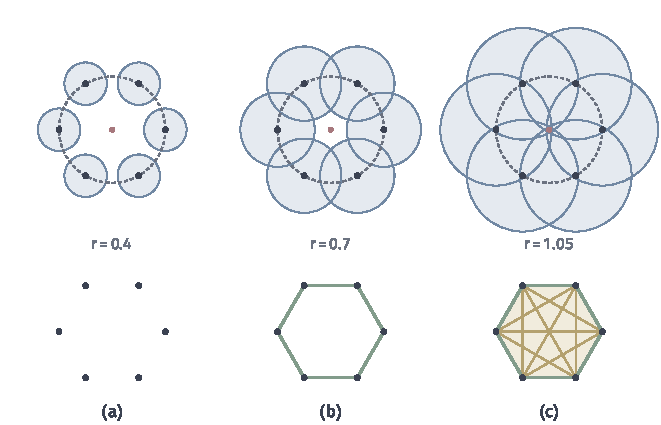
\includegraphics[width=112mm]{figures/04-spaces-measures-and-geometry/04-manifolds/matplotlib/mrec-hexagon/figure.pdf}
  \caption{单位圆上正六边形样本的球并（第一行）与对应的Čech复形（第二行）。虚线是单位圆，红点是圆心。(a) 六个球互不相交，复形只有六个顶点。(b) 相邻的球交叠成环，圆心未被覆盖，复形是六边形的边界。(c) 每个球都含圆心，复形的所有子集都是单纯形（浅黄表示填充），洞消失。}
  \label{fig:mrec-hexagon}
\end{BookInlineFigure}

\subsection{Čech复形}
\label{sec:mrec-cech}

球并是连续空间，不能直接放进计算机。它的拓扑由球与球怎样交叠决定，而交叠关系是有限的组合数据：哪些球两两相交，哪些三个球有公共点，等等。

\begin{definition}[Čech复形]
\label{def:mrec-cech}
给定欧氏空间中的有限点集$P$与半径$r>0$，\term{Čech复形}（Čech complex）$\check C_r(P)$由所有满足$\bigcap_{\bm p\in\sigma}B(\bm p,r)\neq\varnothing$的非空子集$\sigma\subseteq P$组成，其中$B(\bm p,r)$是开球。
\end{definition}

若一组球有公共点，其中任意几个球也有，所以$\check C_r(P)$对取子集封闭，是第~\ref{chap:homology}章意义下的抽象单纯复形。条件$\bigcap_{\bm p\in\sigma}B(\bm p,r)\neq\varnothing$等价于存在一点到$\sigma$中每个点的距离都小于$r$，即覆盖$\sigma$的最小闭球半径小于$r$。特别地，两点连边当且仅当它们的距离小于$2r$。

Čech复形记录的是整个球族的交叠，不只是两两的交叠。取边长为$0.9$的正三角形，$r=0.5$，如图~\ref{fig:mrec-cech-rips}。三对球两两相交，因为$0.9<1$；但覆盖三个顶点的最小球是外接球，半径
\[
 \frac{0.9}{\sqrt3}\approx0.520>0.5,
\]
三个球没有公共点。所以$\check C_{0.5}$只有三条边，没有三角形，留下一个一维的环；$r$增大到超过$0.520$时三角形被填上，环随之消失。$r\leq r'$时$\check C_r\subseteq\check C_{r'}$，尺度变化改变的正是这种填充关系。

回到正六边形，把顶点依次编号为$0,\ldots,5$。$\tfrac12<r\leq\tfrac{\sqrt3}2$时复形是六边形的边界。$r$超过$\tfrac{\sqrt3}2$后，隔一个顶点的两点连边，三个相邻顶点组成的三角形也被填上，但这些三角形都贴着外圈，中间的洞还在；直到$r>1$时，含对径点的单纯形和三角形$\{0,2,4\}$、$\{1,3,5\}$才出现，把洞填上。复形的同调与球并的同调随$r$同步变化，这不是巧合，第~\ref{sec:mrec-nerve-lemma}节解释原因。

\subsection{Rips复形}
\label{sec:mrec-rips}

判断三个以上的球有没有公共点，需要计算最小覆盖球，在高维中代价不小，而且要用到点的坐标。只用成对距离的替代方案是Rips复形。

\begin{definition}[Rips复形]
\label{def:mrec-rips}
给定有限点集$P$与它们之间的距离，以及$r>0$，\term{Rips复形}（Vietoris--Rips complex）$R_r(P)$由所有直径不超过$r$的非空子集$\sigma\subseteq P$组成，即$\sigma$中任意两点的距离都不超过$r$。
\end{definition}

判定一个单纯形只需要它各顶点之间的成对距离，所以Rips复形可以直接由距离表构造，不需要坐标，也不需要距离来自欧氏点。它由边完全确定：一组顶点构成单纯形，当且仅当其中两两之间都有边。这既是计算上的便利，也意味着它丢失了“成对相交而无公共点”的区别。

\begin{BookInlineFigure}
  \centering
  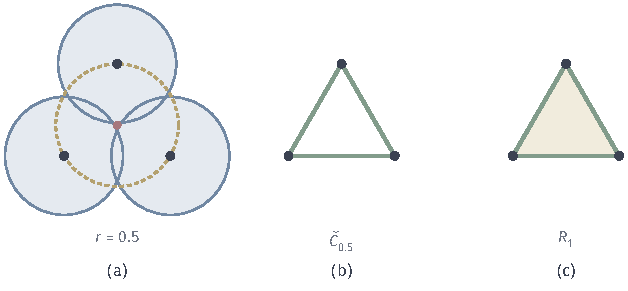
\includegraphics[width=106.299mm]{figures/04-spaces-measures-and-geometry/04-manifolds/tikz/mrec-cech-rips/figure.pdf}
  \caption{边长$0.9$的正三角形。(a) 半径$0.5$的三个球两两相交，但没有公共点；虚线是半径约$0.520$的外接圆，圆心（红）在三个开球之外。(b) Čech复形$\check C_{0.5}$只有三条边，中间是空的。(c) Rips复形$R_1$只看成对距离，三边都不超过$1$，三角形被填上。}
  \label{fig:mrec-cech-rips}
\end{BookInlineFigure}

比较两种复形时，要注意参数的含义不同：Čech复形的$r$是开球半径，Rips复形的$r$是闭的直径界。在上例中，$R_1$含有那个三角形，$\check C_{0.5}$不含，二者连边的条件几乎相同，却不是同一个复形。两者之间有如下的夹逼关系：对任意$\eta>0$，
\begin{equation}
 \check C_r(P)\subseteq R_{2r}(P)\subseteq\check C_{2r+\eta}(P).
 \label{eq:mrec-cech-rips}
\end{equation}

第一个包含：若$\sigma$中各点到某个$\bm z$的距离都小于$r$，则任意两点距离小于$2r$。第二个包含：若$\sigma$的直径不超过$2r$，取$\sigma$中任一顶点作为公共点，它到其余顶点的距离不超过$2r<2r+\eta$。这些常数足以使用，但不是最紧的。夹逼关系说明两种复形在尺度相差一倍的范围内相互控制，不能在同一个数值参数下直接等同。

\subsection{神经引理}
\label{sec:mrec-nerve-lemma}

Čech复形是球并的组合记录，现在要说明这一记录没有丢失同伦信息。一般地，给定一族集合，可以只记录哪些成员有公共点。

\begin{definition}[神经与良覆盖]
\label{def:mrec-nerve}
设$\mathcal U=\{U_1,\ldots,U_n\}$是一族集合。它的\term{神经}（nerve）$N(\mathcal U)$是以$\{1,\ldots,n\}$为顶点集的抽象单纯复形，非空子集$\sigma$是单纯形当且仅当$\bigcap_{i\in\sigma}U_i\neq\varnothing$。若每个非空的有限交$\bigcap_{i\in\sigma}U_i$都是可缩空间，则称$\mathcal U$为\term{良覆盖}（good cover），这里覆盖指它覆盖并集$\bigcup_iU_i$。
\end{definition}

按定义，$\check C_r(P)$就是开球族$\{B(\bm p,r)\}_{\bm p\in P}$的神经。有限个欧氏开球构成良覆盖：凸集的交仍是凸集，非空凸集$K$可以沿直线收缩到其中一点$\bm z_0$，同伦取
\[
 H(\bm x,t)=(1-t)\bm x+t\bm z_0 ,
\]
凸性保证$H(\bm x,t)\in K$，所以$K$可缩。

\begin{theorem}[神经引理]
\label{thm:mrec-nerve-lemma}
设$\mathcal U$是$\mathbb R^D$中有限个开凸集组成的族，则神经的几何实现$\lvert N(\mathcal U)\rvert$与并集$\bigcup_iU_i$同伦等价。特别地，对有限点集$P$和任意$r>0$，$\lvert\check C_r(P)\rvert$与球并$U_r$同伦等价。
\end{theorem}

完整的证明较长，读者可查阅Hatcher《代数拓扑》中关于神经的推论。这里构造两个方向的映射，并验证其中一个复合同伦于恒等映射，这已经能看出凸性起的作用。

从并集到神经：取一组连续函数$\varphi_i\geq0$，在$U_i$内为正、在$U_i$外为零，且处处$\sum_i\varphi_i=1$，例如把$\bm x$到$U_i$补集的距离归一化。令$F(\bm x)=\sum_i\varphi_i(\bm x)\bm v_i$，$\bm v_i$是第$i$个顶点。$\varphi_i(\bm x)>0$的那些$i$对应的集合都含$\bm x$，有公共点，所以$F(\bm x)$落在神经中的一个单纯形内。

反方向，在每个非空交$\bigcap_{i\in\sigma}U_i$中取一点$\bm c_\sigma$，在$\lvert N(\mathcal U)\rvert$的重心细分上，把$\sigma$的重心送到$\bm c_\sigma$，再在细分的每个单纯形上线性延拓，得到$G$。细分中的单纯形对应一串$\sigma_0\subseteq\cdots\subseteq\sigma_k$，所有$\bm c_{\sigma_j}$都在凸集$\bigcap_{i\in\sigma_0}U_i$中，所以$G$的像落在并集内。

现在看$G\circ F\simeq\mathrm{id}$。设$F(\bm x)$落在细分单纯形$\sigma_0\subseteq\cdots\subseteq\sigma_k$内，此时$\sigma_k$中的每个集合都含$\bm x$，特别是$\sigma_0$中的每个集合都含$\bm x$。于是$\bm x$与$G(F(\bm x))$都在凸集$\bigcap_{i\in\sigma_0}U_i$中，连接它们的线段也在其中，直线同伦$(1-t)\bm x+tG(F(\bm x))$就留在并集内。

另一个复合$F\circ G$同伦于恒等映射，这一步要复杂得多，需要在神经上逐层构造同伦，完整的论证见上面所指的文献。

神经引理把连续空间的问题转为有限计算。由第~\ref{chap:homology}章的同伦不变性，同伦等价的空间有同构的同调，几何实现的同调又等于单纯同调，于是
\begin{equation}
 H_k(U_r)\cong H_k\bigl(\lvert\check C_r(P)\rvert\bigr)\cong H_k\bigl(\check C_r(P)\bigr),
 \label{eq:mrec-nerve-homology}
\end{equation}
右端只需写出$\check C_r(P)$的边界矩阵并计算秩。正六边形的例子正是这样：$\tfrac12<r\leq\tfrac{\sqrt3}2$时，复形是六个顶点、六条边的环，边界矩阵的秩为$5$，$\beta_1=6-5=1$，与球并的环对应。

\subsection{恢复尺度}
\label{sec:mrec-recovery-scale}

至此，球并的同调可以由Čech复形算出。剩下的问题是：球并的同调何时等于$M$的同调？回到第~\ref{sec:mrec-ball-union}节的六边形，半径太小时球并断开，太大时洞被填掉，需要一个既不太小也不太大的半径。

\paragraph{两类条件}

第一类条件是覆盖：$M\subseteq U_r$，否则流形上未被覆盖的部分会让球并断开或多出洞。若样本是$\delta$稠密的，$r\geq\delta$即可。

第二类条件是不错误地连接或填充：球并不能把流形相距较远的部分接起来，也不能把流形围出的洞盖住。由于球心都在$M$上，$U_r$中每一点到$M$的距离小于$r$；若$r<\tau$，$U_r\subseteq M^\tau$，最近点投影$\pi$在整个$U_r$上有定义。

两类条件写成同一个半径的允许范围：$r$要大于某个由覆盖精度决定的下界，又要小于某个由可达半径决定的上界。只有覆盖精度相对可达半径足够小时，这个范围才非空。只看样本很密，或只看球并连通，都推不出恢复：六边形样本在$r=1.01$时球并连通且包含圆，同调却已与圆不同。

\paragraph{形变收缩的前提}

要证明$U_r$与$M$有同样的同调，最自然的方法是把$U_r$形变收缩到$M$上：令
\begin{equation}
 F(\bm x,t)=(1-t)\bm x+t\,\pi(\bm x),
 \label{eq:mrec-retraction}
\end{equation}
把每一点沿直线推向它的最近点，如图~\ref{fig:mrec-retraction}(a)。$t=0$时是恒等映射，$t=1$时落在$M$上，$M$上的点始终不动。第~\ref{chap:homology}章说明形变收缩是同伦等价。

这一构造需要两个前提。一是$\pi$在$U_r$上有定义且连续，由$r<\tau$保证。二是从$\bm x$到$\pi(\bm x)$的线段整个留在$U_r$中，否则$F$会离开$U_r$，不是$U_r$上的形变。第二个前提并不平凡：线段从$\bm x$所在的球出发，它的另一端$\pi(\bm x)$可能落在别的球里，中间不能经过球并之外的缝隙。下一小节的证明处理的就是这件事。

\paragraph{圆上的核对}

单位圆的可达半径为$\tau=1$。下一小节的定理要求样本是$\varepsilon/2$稠密的，且$\varepsilon<\sqrt{3/5}\,\tau\approx0.775$，所以覆盖精度必须小于约$0.387$。

正六边形的覆盖精度是$0.518$，不满足条件。尽管如此，$r=0.6$时球并覆盖了圆，又没有盖住圆心，同调仍然正确；定理的条件是充分的，不是必要的。

改取$24$个等距样本，覆盖精度为$0.131$。允许的半径范围是$2\times0.131<\varepsilon<0.775$，例如$\varepsilon=0.3$，图~\ref{fig:mrec-retraction}(a)画的就是这个球并。在这个范围内，定理保证球并的同调等于圆的同调，即$\beta_0=\beta_1=1$。

\subsection{同调恢复定理}
\label{sec:mrec-homology-theorem}

把上面的条件定量化，就得到Niyogi、Smale与Weinberger的结果。

\begin{theorem}[有限样本的同调恢复]
\label{thm:mrec-homology-recovery}
设$M\subseteq\mathbb R^D$是紧致无边界的光滑嵌入子流形，可达半径为$\tau>0$。设有限样本$P\subseteq M$是$\varepsilon/2$稠密的，即$M$上每一点到最近样本的环境距离小于$\varepsilon/2$，且$0<\varepsilon<\sqrt{3/5}\,\tau$。则式~\eqref{eq:mrec-ball-union}的球并$U_\varepsilon$形变收缩到$M$，从而对每个$k$，
\begin{equation}
 H_k(M)\cong H_k(U_\varepsilon)\cong H_k\bigl(\check C_\varepsilon(P)\bigr).
 \label{eq:mrec-homology-recovery}
\end{equation}
\end{theorem}

证明的关键是说明线段$[\bm x,\pi(\bm x)]$留在球并中。思路是分两种情形：要么$\pi(\bm x)$就在$\bm x$所在的球内，线段自然留在这个凸的球里；要么$\pi(\bm x)$离球心较远，这时可以证明$\bm x$离流形很近，于是整条线段都落在$\pi(\bm x)$附近某个样本的球里，如图~\ref{fig:mrec-retraction}(b)。

\begin{proof}
由$\varepsilon/2$稠密，$M\subseteq U_\varepsilon$。由$\varepsilon<\tau$，$U_\varepsilon\subseteq M^\tau$，$\pi$在$U_\varepsilon$上连续。下面证明对任一$\bm x\in U_\varepsilon$，线段$[\bm x,\pi(\bm x)]$留在$U_\varepsilon$中。

设$\bm x\in B(\bm p,\varepsilon)$，$\bm p\in P$。记$\bm q=\pi(\bm x)$，并记
\[
 T=\lVert\bm x-\bm q\rVert_2,\qquad a=\lVert\bm p-\bm q\rVert_2 .
\]
$T=0$时无需证明。否则令$\bm v=(\bm x-\bm q)/T$，由一阶条件它是$\bm q$处的单位法向量。$\bm q$是最近点，所以
\[
 T\leq\lVert\bm x-\bm p\rVert_2<\varepsilon<\tau .
\]

情形一，$a<\varepsilon$。此时$\bm x,\bm q$都在开球$B(\bm p,\varepsilon)$中，球是凸的，线段留在其中。

情形二，$a\geq\varepsilon$。先估计$T$。由$\bm x-\bm p=(\bm q-\bm p)+T\bm v$，
\[
 \lVert\bm x-\bm p\rVert_2^2=a^2+T^2-2T\langle\bm p-\bm q,\bm v\rangle .
\]
由式~\eqref{eq:mrec-reach-normal}，$\langle\bm p-\bm q,\bm v\rangle\leq a^2/(2\tau)$，代入并用$\lVert\bm x-\bm p\rVert_2<\varepsilon$，得
\[
 \varepsilon^2>a^2\Bigl(1-\frac T\tau\Bigr)+T^2 .
\]
因为$T<\tau$，右端对$a$递增，代入$a\geq\varepsilon$，得$\varepsilon^2>\varepsilon^2(1-T/\tau)+T^2$，整理后
\begin{equation}
 T<\frac{\varepsilon^2}\tau .
 \label{eq:mrec-t-bound}
\end{equation}

再取样本$\bm q'$使$b=\lVert\bm q-\bm q'\rVert_2<\varepsilon/2$，这由稠密性保证。线段上的点可写成$\bm y=\bm q+t\bm v$，$0\leq t\leq T$。展开$\lVert\bm y-\bm q'\rVert_2^2$，并对$\bm q'-\bm q$的法向分量用式~\eqref{eq:mrec-reach-normal}，得
\[
 \lVert\bm y-\bm q'\rVert_2^2\leq b^2+t^2+\frac{tb^2}\tau .
\]
代入$b^2<\varepsilon^2/4$和式~\eqref{eq:mrec-t-bound}，
\[
 \lVert\bm y-\bm q'\rVert_2^2<\frac{\varepsilon^2}4+\frac{\varepsilon^4}{\tau^2}+\frac{\varepsilon^4}{4\tau^2}=\frac{\varepsilon^2}4+\frac54\cdot\frac{\varepsilon^4}{\tau^2}.
\]
由$\varepsilon^2<\tfrac35\tau^2$，第二项小于$\tfrac34\varepsilon^2$，于是$\lVert\bm y-\bm q'\rVert_2<\varepsilon$。整条线段都在球$B(\bm q',\varepsilon)$中。

这样，式~\eqref{eq:mrec-retraction}定义的$F$就是$U_\varepsilon$到$M$的形变收缩：它连续，$t=0$时是恒等映射，$t=1$时映入$M$，且保持$M$上的点不动。所以$M\hookrightarrow U_\varepsilon$是同伦等价，第一个同构成立。第二个同构是式~\eqref{eq:mrec-nerve-homology}。
\end{proof}

常数$\sqrt{3/5}$的来源就在这个证明里：它恰好使$\tfrac14+\tfrac54(\varepsilon/\tau)^2<1$。右端是有限复形的单纯同调，可以由边界矩阵的秩算出，这就是“由有限样本恢复同调”的含义。

\begin{BookInlineFigure}
  \centering
  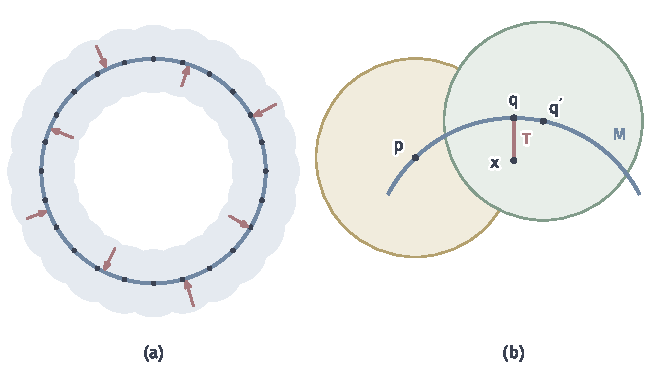
\includegraphics[width=112mm]{figures/04-spaces-measures-and-geometry/04-manifolds/matplotlib/mrec-retraction/figure.pdf}
  \caption{球并向流形的形变收缩。(a) 单位圆上$24$个等距样本、$\varepsilon=0.3$的球并（浅蓝），红色箭头把点沿线段推向最近点。(b) 证明情形二的几何（$\tau=1$，$\varepsilon=0.7$）：$\bm x$在$\bm p$的球（浅黄）中，但最近点$\bm q$不在其中；此时$T<\varepsilon^2/\tau$，线段$[\bm x,\bm q]$整条落在靠近$\bm q$的样本$\bm q'$的球（浅绿）中。}
  \label{fig:mrec-retraction}
\end{BookInlineFigure}

\paragraph{恢复的是什么}

定理恢复的是同调，而且是经由同伦等价得到的。它不给出与$M$同胚的空间：$U_\varepsilon$是$\mathbb R^D$中的开集，维数是$D$而不是$m$，与$M$同伦等价却不同胚；$\check C_\varepsilon(P)$可以含有维数远高于$m$的单纯形。至于$M$的光滑结构、度量或嵌入方式，定理没有给出任何信息。

定理的条件也划定了它的适用范围。样本必须在$M$上：观测离开流形时，需要把扰动界与覆盖精度、可达半径一起放进新的条件，并重新证明形变收缩。定理用的是Čech复形：改用Rips复形时，只能借助式~\eqref{eq:mrec-cech-rips}，在相差一倍的两个尺度之间比较，需要另行论证。从同调进一步恢复同胚类型，则需要完全不同的工具。
